\documentclass{article}

\usepackage{graphicx}
\usepackage{subfigure}
\usepackage[hypcap]{caption}
\usepackage{listings}
\usepackage{float}
\floatstyle{plaintop}
\restylefloat{table}

\title{Experimental Design and Data Analysis: Assignment 4}
\author{Andrew Bedard(2566978) \& Simone van Gompel(2567525) \\ Group 19}

\begin{document}

  \maketitle

  \section*{Exercise 1}
    \subsection*{1}
      \begin{lstlisting}[language=R]
      sample_slices = sample(1:18, 18)
      \end{lstlisting}
    
    \subsection*{2}
      \begin{figure}[H]
          \centering
          \subfigure[Humidity]
          {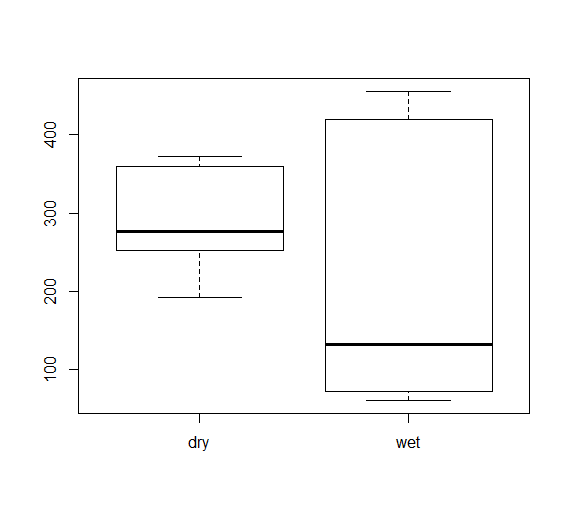
\includegraphics[scale=0.2]{../results/BoxHoursHum.png} }
          \subfigure[Environment]
          {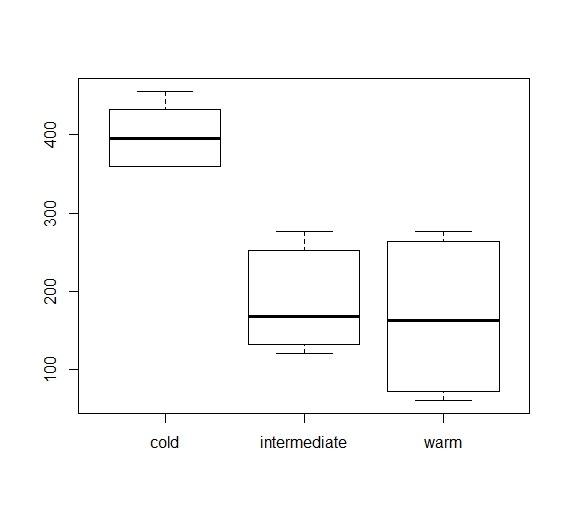
\includegraphics[scale=0.2]{../results/BoxHoursEnv.png} }
          \caption{Boxplots of Hours with Humidity and Environment}
          \label{fig:BoxHours}
      \end{figure} 
    
    \subsection*{3}
      \begin{figure}[H]
          \centering
          \subfigure[Humidity]
          {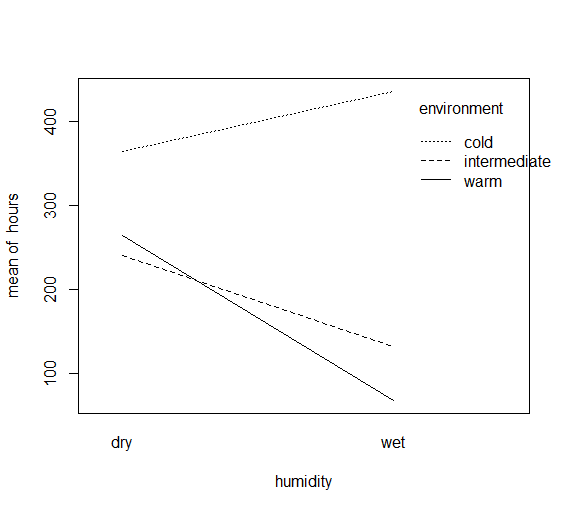
\includegraphics[scale=0.2]{../results/IntPlotHoursHum.png} }
          \subfigure[Environment]
          {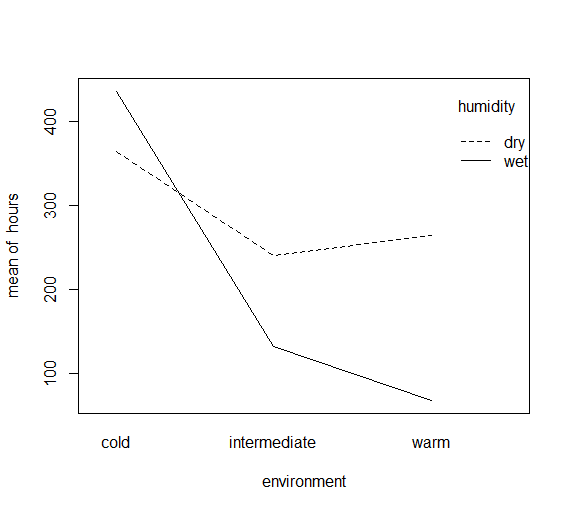
\includegraphics[scale=0.2]{../results/IntPlotHoursEnv.png} }
          \caption{Interactionplots of Hours with Humidity and Environment}
          \label{fig:IntPlotHours}
      \end{figure}
    
    \subsection*{4}
      \begin{lstlisting}[language=R]
Analysis of Variance Table

Response: hours
                     Df Sum Sq Mean Sq F value    Pr(>F)    
environment           2 201904  100952 233.685 2.461e-10 ***
humidity              1  26912   26912  62.296 4.316e-06 ***
environment:humidity  2  55984   27992  64.796 3.705e-07 ***
Residuals            12   5184     432                      
---
      \end{lstlisting}
    
    \subsection*{5}
      The interaction effect of both factors are significant.
      This means that they don't have an additive effect on each other.
      So if you change both the factors, it will have a negative effect on the hours.
    
    \subsection*{6}
      The environment has the biggest numerical influence.
      This is not a good question, it is always better to look at the relative influence of a factor.
    
    \subsection*{7}
      In Fig\ref{fig:QQRes} the QQ-plot of the residuals is shown.
      Here you can see that the data is roughly normally distributed.
      Only the most left and right data points seem to be out of place.
      \begin{figure}[H]
          \centering
          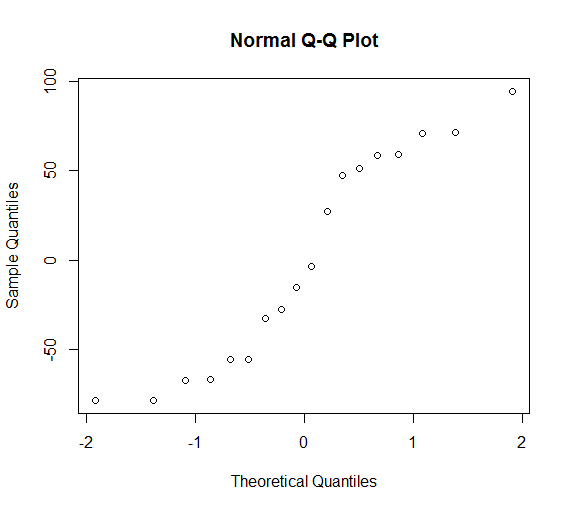
\includegraphics[scale=0.4]{../results/QQResEnvHum.png} 
          \caption{QQ-plot of the residuals}
          \label{fig:QQRes}
      \end{figure}
    
    \subsection*{8}
      In Fig\ref{fig:FitVSRes} the fitted values versus residual values are shown.
      It seems that there is no heteroscedasticity present in this data.
      \begin{figure}[H]
          \centering
          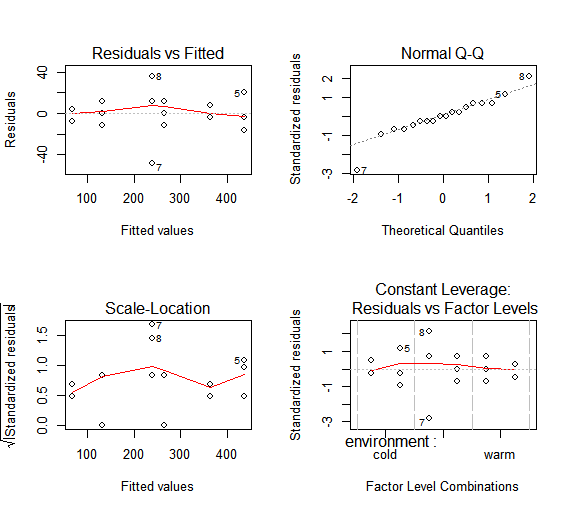
\includegraphics[scale=0.4]{../results/FitVSRes.png} 
          \caption{Fitted Values VS Residual Values}
          \label{fig:FitVSRes}
      \end{figure}
    
    
  \section*{Exercise 2}
    \subsection*{1}
      The used code can be found in \ref{sec:RE2}.
      It makes an array with the numbered students and an array with the skill level of the related student.
      The students are randomly distributed among the three different search engines by using this code:
      \begin{lstlisting}[language=R]
block_design = matrix(c(samples[0:5], 
                        samples[6:10], 
                        samples[11:15]), 
                      nrow = 3, ncol = 5)
      \end{lstlisting}
     
    \subsection*{2}
	\begin{figure}[H]
		\centering
          \subfigure[]
          {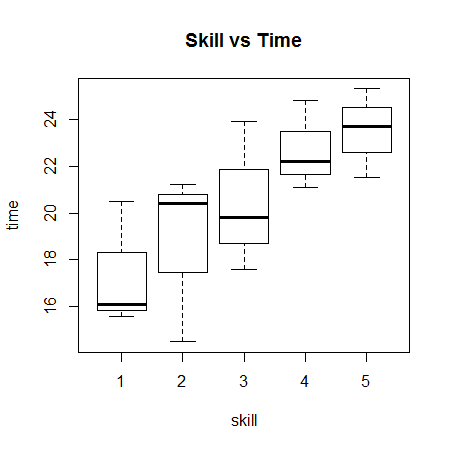
\includegraphics[scale=0.35]{../results/2_2_1.png} }
          \subfigure[]
          {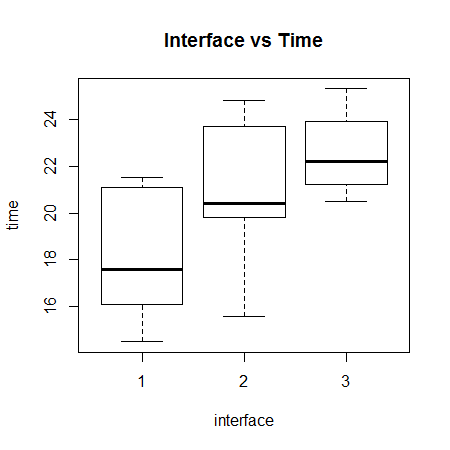
\includegraphics[scale=0.35]{../results/2_2_2.png} }
          \caption{Box Plots of Skill and Interface vs Time}
          \label{fig:srchbox}
	\end{figure}
	
	\begin{figure}[H]
	\centering
		\subfigure[]
          {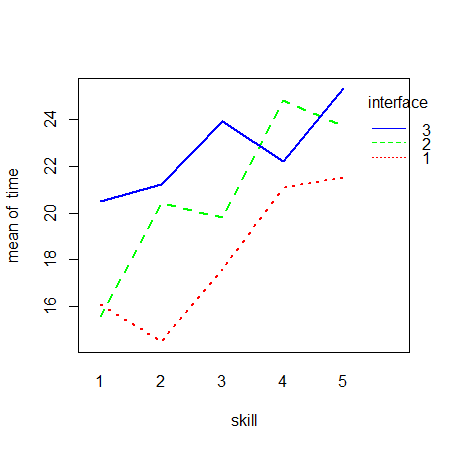
\includegraphics[scale=0.35]{../results/2_2_3.png} }
          \subfigure[]
          {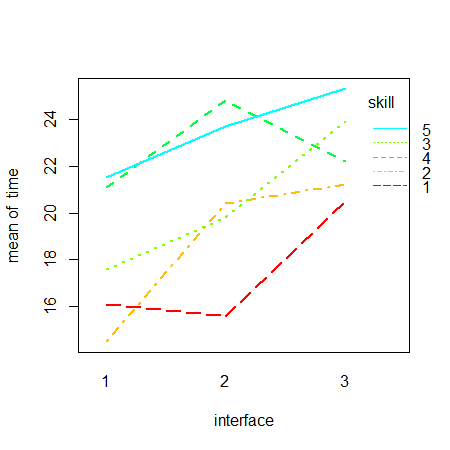
\includegraphics[scale=0.35]{../results/2_2_4.png} }
          \caption{Interaction plots of Skill and Interface vs Time}
          \label{fig:srch_interaction}
	\end{figure}
	
	It is difficult to conclude that there is an interaction between skill and interface as they are clearly not parallel, but they follow the same general trajectory, so this interaction may be due to noise. 
    \subsection*{3}
    Using the Kurskal-Wallis rank sum test, we test if the distributions of our populations in regards to the time measured for different interfaces are the same, and we obtain the following results:\\\\
      \begin{lstlisting}[language=R]
Kruskal-Wallis rank sum test

data: time and interface
Kruskal-Wallis chi-squared = 4.22, df = 2, p-value =0.1212
      \end{lstlisting}
      Thus with a p-value of 0.1212 we reject the null hypothesis that our populations are the same, therefore the search time for all interfaces is not equal.
    \subsection*{4}
    
    \subsection*{5}
    \begin{figure}[H]
    \centering
    	\subfigure[]
		{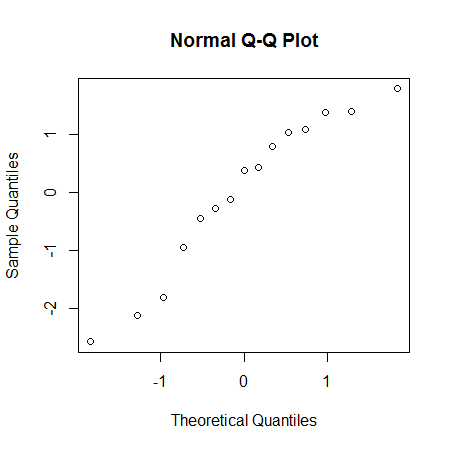
\includegraphics[scale=0.35]{../results/2_5_1.png} }
        \subfigure[]
        {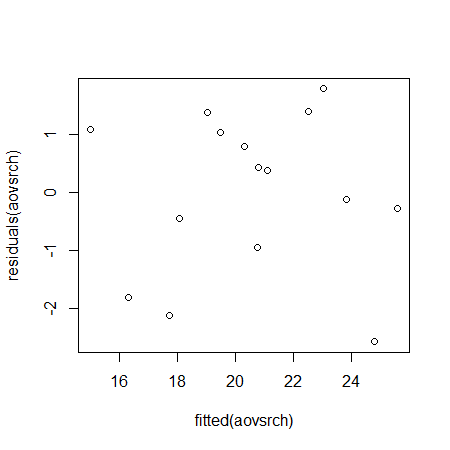
\includegraphics[scale=0.35]{../results/2_5_2.png} }
        \caption{Diagnostic Plots}
        \label{fig:diagnostic}
    \end{figure}
    It is difficult to say for certain, there may be a slight curve in the qq-plot \ref{fig:diagnostic}(a) but it looks approximately normal, and the fitted value plot \ref{fig:diagnostic}(b) suggests there is no significant difference in the population variances.
    \subsection*{6}
	\begin{lstlisting}[language=R]
Friedman rank sum test

data: time, interface and skill
Friedman chi-squared = 6.4, df = 2, p-value = 0.04076
	\end{lstlisting}
	With a p-value of 0.04076 we reject the null hypothesis, thus we conclude there is an effect of interfaces.
    \subsection*{7}
    Testing the null hypothesis that the search time is the same for all interface by a ANOVA test, ignoring skill we obtain the following:
    \begin{lstlisting}[language=R]
    Analysis of Variance Table

Response: time
          Df  Sum Sq Mean Sq F value  Pr(>F)  
interface  2  50.465  25.233  2.8605 0.09642 .
Residuals 12 105.852   8.821                  
---
	\end{lstlisting}
	With a p-value of 0.09642 we do not reject the null hypothesis, thus the time is not the same for all interfaces.
	This test is useful to use, if some conditions are met, as of right now, we do not have convincing evidence there is no interaction between skill and interface. It would be more useful to test along with the variable skill, and the interaction between the two as follows:
	    \begin{lstlisting}[language=R]
	Analysis of Variance Table

Response: time
                Df Sum Sq Mean Sq F value    Pr(>F)    
interface        1 49.729  49.729 21.4145 0.0007313 ***
skill            1 78.732  78.732 33.9039 0.0001154 ***
interface:skill  1  2.312   2.312  0.9956 0.3398204    
Residuals       11 25.544   2.322                      
---
	\end{lstlisting}
	This way we are able to measure the interaction between the data sets, and determine whether there is a factor which has a greater effect on our results. From the previous table we see that with a p-value of 0.3398 we accept the null hypothesis that there is no significant interaction between skill in and interface, which is what we require for the one-way ANOVA ignoring skill to be valid.
  \section*{Exercise 3}
    \subsection*{1}
      \begin{lstlisting}[language=R]
Analysis of Variance Table

Response: acidity
          Df Sum Sq Mean Sq F value   Pr(>F)   
starter    4 44.136 11.0340  8.0835 0.001106 **
batch      1  4.855  4.8547  3.5566 0.078826 . 
position   4  2.348  0.5870  0.4300 0.784786   
Residuals 15 20.475  1.3650                    
      \end{lstlisting}
      
    
    \subsection*{2}
      \begin{lstlisting}[language=R]
Call:
lm(formula = acidity ~ starter + batch + position, data = cream)

Residuals:
    Min      1Q  Median      3Q     Max 
-1.7512 -0.7596  0.0132  0.8816  1.0856 

Coefficients:
            Estimate Std. Error t value Pr(>|t|)    
(Intercept)   7.8260     0.8586   9.115 1.67e-07 ***
starter2     -0.1500     0.7389  -0.203  0.84186    
starter3     -0.9800     0.7389  -1.326  0.20459    
starter4      2.8100     0.7389   3.803  0.00173 ** 
starter5     -0.4840     0.7389  -0.655  0.52238    
batch         0.3116     0.1652   1.886  0.07883 .  
position2    -0.6180     0.7389  -0.836  0.41608    
position3    -0.0380     0.7389  -0.051  0.95966    
position4    -0.7640     0.7389  -1.034  0.31755    
position5    -0.2640     0.7389  -0.357  0.72586    
---

Residual standard error: 1.168 on 15 degrees of freedom
Multiple R-squared:  0.7149,  Adjusted R-squared:  0.5438 
F-statistic: 4.179 on 9 and 15 DF,  p-value: 0.007304
      \end{lstlisting}
      \label{tble:estimates}

    \subsection*{3}
      \begin{lstlisting}[language=R]
Linear Hypotheses:
           Estimate Std. Error t value Pr(>|t|)    
2 - 1 == 0  -0.1500     0.4673  -0.321    0.997    
3 - 1 == 0  -0.9800     0.4673  -2.097    0.282    
4 - 1 == 0   2.8100     0.4673   6.013   <0.001 ***
5 - 1 == 0  -0.4840     0.4673  -1.036    0.834    
3 - 2 == 0  -0.8300     0.4673  -1.776    0.429    
4 - 2 == 0   2.9600     0.4673   6.334   <0.001 ***
5 - 2 == 0  -0.3340     0.4673  -0.715    0.949    
4 - 3 == 0   3.7900     0.4673   8.110   <0.001 ***
5 - 3 == 0   0.4960     0.4673   1.061    0.822    
5 - 4 == 0  -3.2940     0.4673  -7.048   <0.001 ***
      \end{lstlisting}
      \label{tble:p-values}
        Starter 1 and 4 produce significantly different acidity. This is apparent first from exercise 3.2 we obtain: $\mu_1 = 7.8260$ and $\mu_4 = 7.8260 + 2.8100 = 10.636$ which are the estimates for starter 1 and 4 respectively. Furthermore the p-value for starter 1 obtained from exercise 3.2, of 1.67e-07 suggests that we reject the null hypothesis that our estimate for starter 1 is equal to that of the rest of the population, and the p-values obtained from the simultaneous method, of 0.001 suggests that we reject the null hypothesis that the estimate for the treatment effect of 4 is equal to each of the other respective treatment effects.
    \subsection*{4}
    The p-value for the test $H_0: \alpha_2 = \alpha_1$, where $\alpha_i$ is our estimate of the treatment effects is 0.997, whereas in exercise 3.2 our p-value for the null hypothesis $H_0: \alpha_2 = \alpha_1$ is 0.84186. It is no coincidence that the p-value obtained from exercise 3.2, is different from that of the simultaneous calculation, this is due to the fact that when calculating the simultaneous p-values for the null hypothesis  $H_0: \alpha_i = \alpha_1$ we are doing so in such a way that the probability of rejecting any null hypothesis in error is less than 0.5. In contrast to the method used in exercise 3.2, where for every null hypothesis our chance of making such an error is $N*0.05$ where N is the number of possibilities to make such an error. In this way the Simultaneous p-values method gives us a higher confidence in our conclusions.
    \subsection*{5}
      \begin{lstlisting}[language=R]
Linear Hypotheses:
           Estimate lwr     upr    
2 - 1 == 0 -0.1500  -1.6391  1.3391
3 - 1 == 0 -0.9800  -2.4691  0.5091
4 - 1 == 0  2.8100   1.3209  4.2991
5 - 1 == 0 -0.4840  -1.9731  1.0051
3 - 2 == 0 -0.8300  -2.3191  0.6591
4 - 2 == 0  2.9600   1.4709  4.4491
5 - 2 == 0 -0.3340  -1.8231  1.1551
4 - 3 == 0  3.7900   2.3009  5.2791
5 - 3 == 0  0.4960  -0.9931  1.9851
5 - 4 == 0 -3.2940  -4.7831 -1.8049
      \end{lstlisting}
    The confidence intervals for testing all differences $\alpha_j - \alpha_{j'}$ for $(i,i' \in {1,2...,5})$ of the main effects for starter with simultaneous confidence level 95\% are (4-1),(4-2),(4-3),(4-5),(5-4) so all those containing starter 4. This is likely due to the fact that the estimated value for starter 4, which was earlier calculated as 10.636, is so much larger than every other estimate, for example all the confidence intervals for (4-i) are greater than 0, and the one interval (5-4) is less than 0.
  \section*{Exercise 4}
    \subsection*{1}
    Performing ANOVA test using an ordinary fixed effects model fitted with lm, the follow results were obtained:
      \begin{lstlisting}[language=R]
      Analysis of Variance Table

Response: milk
          Df  Sum Sq Mean Sq F value Pr(>F)
treatment  1    0.27   0.269  0.0016 0.9682
order      1   53.52  53.515  0.3268 0.5760
Residuals 15 2456.69 163.779  
      \end{lstlisting}
      
      \begin{lstlisting}[language=R]
 Residuals:
    Min      1Q  Median      3Q     Max 
-16.602 -10.103   0.170   9.431  22.042 

Coefficients:
            Estimate Std. Error t value Pr(>|t|)    
(Intercept)  37.1722     5.4379   6.836 5.64e-06 ***
treatmentB   -0.2444     6.0329  -0.041    0.968    
orderBA      -3.4700     6.0704  -0.572    0.576    
---
Signif. codes:  
0 ‘***’ 0.001 ‘**’ 0.01 ‘*’ 0.05 ‘.’ 0.1 ‘ ’ 1

Residual standard error: 12.8 on 15 degrees of freedom
Multiple R-squared:  0.02142,	Adjusted R-squared:  -0.1091 
F-statistic: 0.1642 on 2 and 15 DF,  p-value: 0.8501   
    \end{lstlisting}
    
    We can conclude from the F-value and p-value of 0.0016 and 0.9682 respectively for the treatment effect on milk production, we do not reject the null hypothesis, therefore there is no treatment effect on milk production. Further we observe that the p-value for the null hypothesis that the individual treatments effects are all greater than 0.05, thus we accept the null hypothesis that the treatment effects are equal. This stands to reason as if we do not conclude there is any effect for all treatments, there would be no effect for individual treatments when sample sizes are equal.
    
    \subsection*{2}
      For the treatment order AB, the summary of milk is:
	\begin{lstlisting}[language=R]
   Min. 1st Qu.  Median    Mean 3rd Qu.    Max. 
  26.50   28.32   34.15   37.05   43.62   54.00 
    \end{lstlisting}
      For the treatment order BA, the summary of milk is:
  \begin{lstlisting}[language=R]
   Min. 1st Qu.  Median    Mean 3rd Qu.    Max. 
  21.40   30.45   37.80   37.56   44.90   55.50  
    \end{lstlisting}
      From these results one can conclude that the cows with the BA order have a higher milk production than the ones with the AB order.

    \subsection*{3}
    \begin{lstlisting}[language=R]
    Analysis of Variance Table
          Df  Sum Sq Mean Sq F value
treatment  1 0.26889 0.26889  0.0503
order      1 0.82889 0.82889  0.1552


     AIC      BIC   logLik deviance df.resid 
   125.4    129.9    -57.7    115.4       13 
   
Scaled residuals: 
     Min       1Q   Median       3Q      Max 
-1.31202 -0.45325 -0.01847  0.33881  1.56294 

Random effects:
 Groups   Name        Variance Std.Dev.
 id       (Intercept) 169.755  13.029  
 Residual               5.341   2.311  
Number of obs: 18, groups:  id, 9

Fixed effects:
            Estimate Std. Error t value
(Intercept)  37.1722     6.5881   5.642
treatmentB   -0.2444     1.0895  -0.224
orderBA      -3.4700     8.8086  -0.394

Correlation of Fixed Effects:
           (Intr) trtmnB
treatmentB -0.083       
orderBA    -0.743  0.000
    \end{lstlisting}

    \subsection*{4}
    \begin{lstlisting}[language=R]
    	Paired t-test

data:  milk[treatment == "A"] and milk[treatment == "B"]
t = 0.2244, df = 8, p-value = 0.8281
alternative hypothesis: true difference in means is not equal to 0
95 percent confidence interval:
 -2.267910  2.756799
sample estimates:
mean of the differences 0.2444444
    \end{lstlisting}

    
  \section{R-Code}
    \subsection{Exercise 1}\label{sec:RE1}
      \begin{lstlisting}[language=R]
bread = read.table("bread.txt")
hours = bread$hours
humidity = bread$humidity
environment = bread$environment

#1.1
sample_slices = sample(1:18, 18)

#1.2
boxplot(hours~humidity)
boxplot(hours~environment)

#1.3
interaction.plot(humidity, environment, hours)
interaction.plot(environment, humidity, hours)

#1.4
aovenvhum = lm(hours ~ environment*humidity, data=bread)
anova(aovenvhum)

#1.7
qqnorm(residuals(aovenvhum))

#1.8
par(mfrow=c(2,2))
plot(aovenvhum)

      \end{lstlisting}
    \subsection{Exercise 2}\label{sec:RE2}
      \begin{lstlisting}[language=R]
#Note: The interface is of greatest importance

search = read.table("search.txt")

time =search$time
skill = search$skill
interface = search$interface

#2.1
students = 1:15
# set the lvls of the students
skill_lvls = rep(c(1,2,3,4,5), each=3)
# sample the students
samples = sample(students, 15)
# make the block_design
block_design = matrix(c(samples[0:5], 
                        samples[6:10], 
                        samples[11:15]), 
                      nrow = 3, ncol = 5)
skill_block_design = matrix(c(skill_lvls[samples[0:5]], 
                              skill_lvls[samples[6:10]], 
                              skill_lvls[samples[11:15]]), 
                            nrow = 3, ncol = 5)

#2.2


boxplot(time~skill,xlab="skill",ylab="time", main="Skill vs Time")
boxplot(time~interface,xlab="interface",ylab="time", main="Interface vs Time")

interaction.plot(skill,interface,time,lwd=2,col=rainbow(3))
interaction.plot(interface,skill,time,lwd=2,col=rainbow(8))

#2.3
interface = factor(search$interface)
skill = factor(search$skill)
kruskal.test(time,interface)

#2.4

aovsrch=lm(time~skill+interface)
summary(aovsrch)

#2.5

qqnorm(residuals(aovsrch))
plot(fitted(aovsrch),residuals(aovsrch))

#2.6

friedman.test(time,interface,skill)

#2.7
anovinter = lm(time~interface)
anova(anovinter)

anv = lm(time~interface*skill,data=search)
anova(anv)
      \end{lstlisting}
    \subsection{Exercise 3}\label{sec:RE3}
      \begin{lstlisting}[language=R]
library(multcomp)

cream = read.table("cream.txt",header=T)
cream$starter = factor(cream$starter)
cream$position = factor(cream$position)

#3.1

anovacid = lm(acidity~starter+batch+position,data=cream)
anova(anovacid)

#3.2
summary(anovacid)

#3.3
tmp = glht(creamlm, linfct=mcp(starter="Tukey"))
summary(tmp)

#3.4
confint(tmp)
      \end{lstlisting}
    \subsection{Exercise 4}\label{sec:RE4}
      \begin{lstlisting}[language=R]
library(lme4)

cow = read.table("cow.txt",header=T)
cow$order = factor(cow$order)
order = cow$order
milk = cow$milk
cow$treatment = factor(cow$treatment)
treatment = cow$treatment

#4.1
cowlm = lm(milk ~ treatment + order, data=cow)
anova(cowlm)
summary(cowlm)

#4.2
summary(cow[0:8,]$milk)
summary(cow[9:16,]$milk)

#4.3
cowlmer = lmer(milk ~ treatment + order+(1|id), data=cow)
anova(cowlmer)
summary(cowlmer)

#4.4
attach(cow)
t.test(milk[treatment=="A"],milk[treatment=="B"],paired=TRUE)

      \end{lstlisting}
\end{document}
